
%(BEGIN_QUESTION)
% Copyright 2007, Tony R. Kuphaldt, released under the Creative Commons Attribution License (v 1.0)
% This means you may do almost anything with this work of mine, so long as you give me proper credit

Examine this water filter control system, then answer the following questions:

$$\includegraphics[width=15.5cm]{i01811x01.eps}$$

\begin{itemize}
\item{} Identify all primary and secondary (cascaded) loops.
\item{} The necessary control actions (direct/reverse) for each controller, assuming direct-acting transmitters and signal-to-open valve actuators.
\item{} What will happen to the filter water level if the influent supply suddenly shuts off?
\item{} What will happen to the clearwell reservoir water level if the influent supply suddenly shuts off?
\end{itemize}

\vskip 20pt \vbox{\hrule \hbox{\strut \vrule{} {\bf Suggestions for Socratic discussion} \vrule} \hrule}

\begin{itemize}
\item{} A useful analytical technique for any complex control system is to annotate the diagram with ``+'' and ``$-$'' symbols at the instrument bubble inputs, designating ``noninverting'' and ``inverting'' characteristics, respectively.  Show how this helps you track of all directions of action, making it easier to figure out how the control system responds to changes.
\item{} Explain what will happen in this system if the clearwell inlet flow transmitter fails with a low signal.
\item{} Explain what will happen in this system if the clearwell inlet flow transmitter fails with a high signal.
\item{} Explain what will happen in this system if the clearwell level transmitter fails with a low signal.
\item{} Explain what will happen in this system if the clearwell level transmitter fails with a high signal.
\item{} For those who have studied PID tuning, what PID tuning parameters (qualitative) would you recommend for each controller in this system?
\end{itemize}

\underbar{file i01811}
%(END_QUESTION)





%(BEGIN_ANSWER)

\noindent
{\bf Partial answer:}

\vskip 10pt

Both flow controllers must be {\it reverse-acting}.  Both level controllers must also be {\it reverse-acting}.  In the event of a water supply failure, both levels will fail low (become empty).

%(END_ANSWER)





%(BEGIN_NOTES)

The flow controllers are secondary (slave) loops to the primary (master) level controllers.  








\vfil \eject

\noindent
{\bf Prep Quiz:}

Identify the necessary control action directions (i.e. {\it direct} or {\it reverse}) for each of the two level controllers in this cascade control system.  State a separate answer for both LIC-22 and LIC-28, assuming signal-to-open control valves in each case:

$$\includegraphics[width=15.5cm]{i01811x02.eps}$$

\vfil \eject

\noindent
{\bf Prep Quiz:}

Identify which controllers are {\it masters} and which controllers are {\it slaves} in this cascade control system:

$$\includegraphics[width=15.5cm]{i01811x02.eps}$$


%INDEX% Control, strategies: cascade
%INDEX% Process: water filter flow/level control

%(END_NOTES)


